%! Author = Stepan Oskin
%! Date = 2019-08-01

% Preamble
\documentclass[11pt]{article}
\usepackage{graphicx}

% Packages

% Document
\begin{document}

    \title{GTHA housing market database \\
    OSEMN methodology \\
    Step 2: Scrub (clean) data \\
    Cleanup plan for the Teranet dataset}

    \author{Stepan Oskin}

    \maketitle

    \begin{abstract}
        Teranet dataset plays an integral part in the proposed GTHA housing market database, design and implementation of which is the primary focus of this Master Thesis.
        In order to allow the implementation of constraints dictated by the database design, as well as for facilitation of future analysis and modelling based on the database information, it is critical to ensure particular structure and certain degree of consistency of the input data.
        To address this issue, this document outlines the cleanup plan for the Teranet dataset.

        The four main steps of the cleanup process include: spatial join of Teranet points with the polygons of Dissemination Areas, correction of inconsistent entries, addition of new attributes, and removal of duplicated transactions.
        Additional steps may include: filtering transactions for low and high outliers based on the values of \texttt{consideration\_amt}, correction of \texttt{consideration\_amt} for inflation to ensure consistency of dollar values across time, and normalization of values in \texttt{consideration\_amt}.
    \end{abstract}

    \section{Introduction} \label{sec:teranet_cleaning_intro}

    This document presents \textit{Step 2: Scrub} of OSEMN methodology for data science projects.
    For detailed description of OSEMN methodology, see \\ \texttt{methodology/0.osemn/osemn.pdf}.

    \vspace{5mm}

    For background information, description of the Teranet dataset, and its attributes, see \texttt{methodology/1.obtain/obtain.pdf}.

    \vspace{5mm}

    As outlined in the document \textit{Step 2: Scrub (clean) data} (see \\ \texttt{methodology/2.scrub/scrub.pdf} for details), data analytics, statistical models, and machine learning algorithms, in order to produce meaningful results, require input data to be consistent and transformed into an appropriate form.

    In addition to that, as outlined in the \textit{Description of Relational Databases} (see \texttt{methodology/rdbms/rdbms.pdf} for details), the main idea of a database is to force the data into a certain structure to allow implementation of constraints and relationships between entities.
    Organizing data in such a way allows for reduction of redundancy in data storage and drastic improvement in efficiency when working with related datasets.
    Thus, input data for a relational database also needs to be consistent in order for constraints and relations to work properly.

    Data also needs to follow the ''tidy'' format, as described in section~\ref{sec:db_norm_tidy_data} of this document.
    Teranet dataset is mostly ''tidy'' in its structure, but does have multiple issues with its consistency, such as inconsistent spelling, multiple attributes recorded in a single column (some records have their \texttt{unitno}, \texttt{street\_number}, \texttt{postal\_code}, \texttt{street\_designation} and/or \texttt{street\_direction} recorded as parts of their \texttt{street\_name}), missing and erratic values, and duplicate records.
    This document describes the steps taken to address these issues, in order to improve the quality and usability of the Teranet dataset, and to meet the requirements needed for the organization of the proposed GTHA housing market database via PostgreSQL .

    \section{Cleanup plan for the Teranet dataset} \label{sec:teranet_cleanup_plan}

    The four main steps of the cleanup process of the Teranet dataset include:
    \begin{itemize}
        \item Step 2.1: spatial join of Teranet points with the polygons of Dissemination Areas (DAs), results in addition of 3 new attributes: \texttt{objectid}, \texttt{dauid}, and \texttt{csdname}.
        Attribute \texttt{dauid} allows the establishment of the relationship between the Teranet records and Dissemination Areas (they can be joined in the future via a non-spatial operation).
        \item Step 2.2: correction of inconsistent entries
        \item Step 2.3: addition of new attributes: \texttt{transaction\_id}, \texttt{price\_disp}, \texttt{year}, and \texttt{decade}
        \item Step 2.4: removal of duplicate records from the Teranet dataset
    \end{itemize}

    \vspace{5mm}

    Additional cleanup steps may include:
    \begin{itemize}
        \item filtering Teranet transactions for low and high outliers based on the values of \texttt{consideration\_amt}
        \item correction of \texttt{consideration\_amt} for inflation to ensure consistency of dollar values across time
        \item normalization of values for \texttt{consideration\_amt}
    \end{itemize}

    \section{Tidy data and database normalization} \label{sec:db_norm_tidy_data}

    This section describes the concept of ''Tidy Data'', as defined by Hadley Wickham.
    The concept of ''Tidy Data'' presents the basic ideas of normalization of a database, as defined by Edgar F. Codd, reformulated in statistical language.

    \subsection{Tidy data} \label{subsec:tidy_data}

    Hadley Wickham in his paper \textit{''Tidy Data''}\cite{Wickham2014} formalized the way how a shape of the data can be described and what goal should be pursued when formatting data.
    The principles of tidy data provide a standard way to organize data values within a dataset.
    The tidy data standard has been designed to facilitate initial exploration and analysis of the data, and to simplify the development of data analysis tools that work well together.
    The principles of tidy data are closely tied to those of relational databases and Codd's relational algebra\cite{Codd1990}.

    As an integral part of his \textbf{relational model}, Codd proposed a process of database normalization, or restructuring of a relational database in accordance with a series of so-called \textbf{normal forms} in order to reduce data redundancy and improve data integrity.

    \subsection{Normalization of a database according to Codd} \label{subsec:db_norm}

    Normalization entails organizing the columns (attributes) and tables (relations) of a database to ensure that their dependencies are properly enforced by database integrity constraints.
    As defined by Codd (\cite{Codd1990}, section 17.5.1), the basic ideas in normalization are to organize the information in a database as follows:

    \begin{enumerate}
        \item Each distinct type of object has a distinct type identifier, which becomes the name of a base relation.
        \item Every distinct object of a given type must have an instance identifier that is unique within the object type;
        this is called its \textbf{primary-key} value.
        \item Every fact in the database is a fact about the object identified by the primary key.
        \item Each such fact contains nothing other than the single-valued immediate properties of the object.
        \item Such facts are collected together in a single relation, if they are about objects of the same type.
        The result is a collection of facts, all of the same type.
    \end{enumerate}

    \subsection{Teranet dataset in the context of a normalized database} \label{subsec:teranet_db_norm}

    Teranet dataset is intended to be used as one of the tables (relations) of the proposed GTHA housing market database that would include other sources of information, such as DA-level demographics, land use information, \textit{etc.}
    In this context, Codd's basic normalization ideas would take the following form:

    \begin{enumerate}
        \item The Teranet dataset (filtered to include only GTHA records) presents a single type of object (relation, or table) \textemdash real estate transactions recorded in the GTHA between 1805-01-06 and 2017-10-11.
        \item Every distinct object (transaction) must have an instance identifier that is unique within the object type, or its primary-key value.
        In case of Teranet dataset, all the native columns, including \texttt{registration\_date}, \texttt{pin}, address information, and \texttt{X} and \texttt{Y} coordinates, have duplicated values present (multiple transactions occurring on the same date, address, coordinates, or under the same pin).
        Thus, no combination of such columns constitute a candidate key, which prompts the addition of a new attribute that can serve as a unique identifier for Teranet records.
        \item A new column \texttt{transaction\_id} is added to the dataset to be used as its primary key;
        it corresponds to the row number of each instance (transaction) in the Teranet dataset (filtered to include only GTHA transactions via a spatial join in Step 2.1, see section~\ref{sec:teranet_da_spatial_join} of this document), ordered from the earliest date to the latest.
        \item Every fact in the database is a fact about the object identified by the primary key.
        This condition is met, as every transaction in Teranet dataset is described by the values found in columns of a single row.
        \item Each such fact contains nothing other than the single-valued immediate properties of the object, all columns in Teranet dataset contain single-valued immediate properties of each transaction.
        \item Such facts are collected together in a single relation, as they are all objects of the same type (a single table of real estate transactions recorded in Ontario).
    \end{enumerate}

    Thus, Teranet dataset fits into a normalized database, with the new attribute \texttt{transaction\_id} as its primary key.

    \subsection{Codd's constraints formed in statistical language by Wickham} \label{subsec:teranet_tidy_data}

    According to Wickham\cite{Wickham2014}, \textit{tidy data} is a standard way of mapping the meaning of a dataset to its structure.
    A dataset is messy or tidy depending on how rows, columns and tables are matched up with observations,
    variables and types.

    \vspace{5mm}

    In tidy data:
    \begin{enumerate}
        \item Each variable forms a column.
        \item Each observation forms a row.
        \item Each type of observational unit forms a table.
    \end{enumerate}

    This is Codd's 3rd normal form\cite{Codd1990}, but with the constraints framed in statistical
    language, and the focus put on a single dataset rather than the many connected datasets common in relational databases.
    \textit{Messy data} is any other arrangement of the data.

    \vspace{5mm}

    According to Wickham, the most common problems with messy datasets are:
    \begin{itemize}
        \item Column headers are values, not variable names.
        \item Multiple variables are stored in one column.
        \item Variables are stored in both rows and columns.
        \item Multiple types of observational units are stored in the same table.
        \item A single observational unit is stored in multiple tables.
    \end{itemize}

    In the Teranet dataset, none of these problems are present, so it presents \textit{tidy data}.

    \section{Step 2.1: Spatial join of Teranet points with Dissemination Area polygons} \label{sec:teranet_da_spatial_join}

    Step 2.1 of the cleaning process of Teranet data involved the spatial join of Teranet points with the polygons of Dissemination Areas (DA).
    Parameters that were used for the spatial join operation were \texttt{how='inner', op='within'}.

    The spatial join was performed to filter out Teranet records whose coordinates fall outside of GTHA .

    In addition to that, three new attributes were produced as a results of the spatial join:
    \begin{itemize}
        \item Dissemination Area attributes \texttt{OBJECTID}, \texttt{DAUID}, and \texttt{CSDNAME} were added to each Teranet record falling within a particular DA polygon.
        \item The added attributes allow for extra quality control of Teranet data by comparing the column \texttt{MUNICIPALITY} of Teranet records with the column \texttt{CSDNAME} associated with DA geometry.
        \item New columns \texttt{OBJECTID} and \texttt{DAUID} allow Teranet records to be joined in the future with DA geometry via a regular (non-spatial) join operation (for example, to be aggregated by DAs), or to add any additional DA-level attributes, such as DA-level demographics, to Teranet records.
        \item These future joins can be performed via regular (non-spatial) join operations, which are much less computationally intensive than a spatial join, and thus can be performed much faster.
    \end{itemize}

    \section{Step 2.2: Correction of inconsistent entries} \label{sec:teranet_correction_inconsistent}

    Step 2.2 of the cleanup process for Teranet data focused on the correction of inconsistent entries.

    \subsection{Common problems with data} \label{subsec:common_data_problems}
    Common problems with data may include:

    \begin{itemize}
        \item Inconsistent column names \\
        Column names can have inconsistent capitalizations and/or bad characters.
        \item Missing data \\
        Missing data needs to be identified and addressed.
        \item Outliers \\
        Outliers can pose a potential problem and need to be investigated.
        \item Duplicate rows \\
        Duplicate rows can bias analysis and need to be found and dropped.
        \item Untidy \\
        Untidy datasets can contain multiple problems, and prevent us from quickly transforming our dataset from one suitable for reporting to a dataset suitable for analysis.
        \item Need to process columns \\
        Columns might need to be processed before they can be used for data analysis.
        \item Column types can signal unexpected data values \\
        Column types can signal the presence of unexpected data values.
    \end{itemize}

    \subsection{Modifications made to Teranet dataset} \label{subsec:teranet_modifications}

    The following modifications have been made to the Teranet dataset:

    \begin{enumerate}
        \item Inconsistent capitalizations were fixed for:
        \begin{itemize}
            \item column names
            \item column \texttt{municipality}
            \item column \texttt{street\_name}
            \item column \texttt{street\_designation}
            \item values in the column \texttt{postal\_code} did not show any problems, but were converted to upper case as a preventive measure
        \end{itemize}
        \item Column \texttt{province} was removed from the Teranet dataset, as all the transaction are recorded in the Province of Ontario
        \item Column \texttt{street\_suffix} has been removed from the dataset, since it is missing 99.99994\% of values (see section~\ref{subsubsec:teranet_missing_values}).
    \end{enumerate}

    \subsubsection{Improper capitalizations} \label{subsubsec:teranet_capitalizations}

    \begin{itemize}
        \item Column names have inconsistent capitalizations.
        \item Values in columns \texttt{street\_name}, \texttt{street\_designation} and \texttt{municipality} have inconsistent capitalizations.
        \item Values in column \texttt{postal\_code} do not show problems, but have been converted to upper case as a preventive measure.
    \end{itemize}

    \subsubsection{Data types} \label{subsubsec:teranet_data_types}

    Data type of column \texttt{unitno} detects as a \texttt{float}, though it should contain \texttt{integer} values.
    This happens due to erratic values being present in column \texttt{unitno}, which is addressed in section~\ref{sec:teranet_correction_inconsistent} of this document.
    After the erratic values are corrected, the column can be converted to \texttt{integer} data type.
    This step is performed when Teranet data is entered into the PostgreSQL database, as Pandas library in Python does not have an efficient representation of \texttt{NaN} (missing) values for \texttt{integer} data type\cite{PandasDevelopmentCommunity2019}.

    Data types of all other columns are detected appropriately, indicating consistency of data types in the Teranet dataset.

    Column \texttt{lro\_num} can be converted to \texttt{category} data type, as it contains only a small range of values.
    But since this conversion does not result in significant memory savings, its type was left as \texttt{integer}.

    \subsubsection{Missing values} \label{subsubsec:teranet_missing_values}

    Number of missing records per column in the Teranet dataset is presented in figure~\ref{fig:teranet_na_counts}.

    \vspace{5mm}

    The following columns have no missing values:

    \begin{itemize}
        \item \texttt{pin}
        \item \texttt{lro\_num}
        \item \texttt{registration\_date}
        \item \texttt{x} and \texttt{y}
    \end{itemize}

    \vspace{5mm}

    The new columns that were added via a spatial join in Step 2.1 have no missing values:

    \begin{itemize}
        \item \texttt{objectid}
        \item \texttt{dauid}
        \item \texttt{csdname}
    \end{itemize}
    \begin{figure}[hbt!]
        \centering
        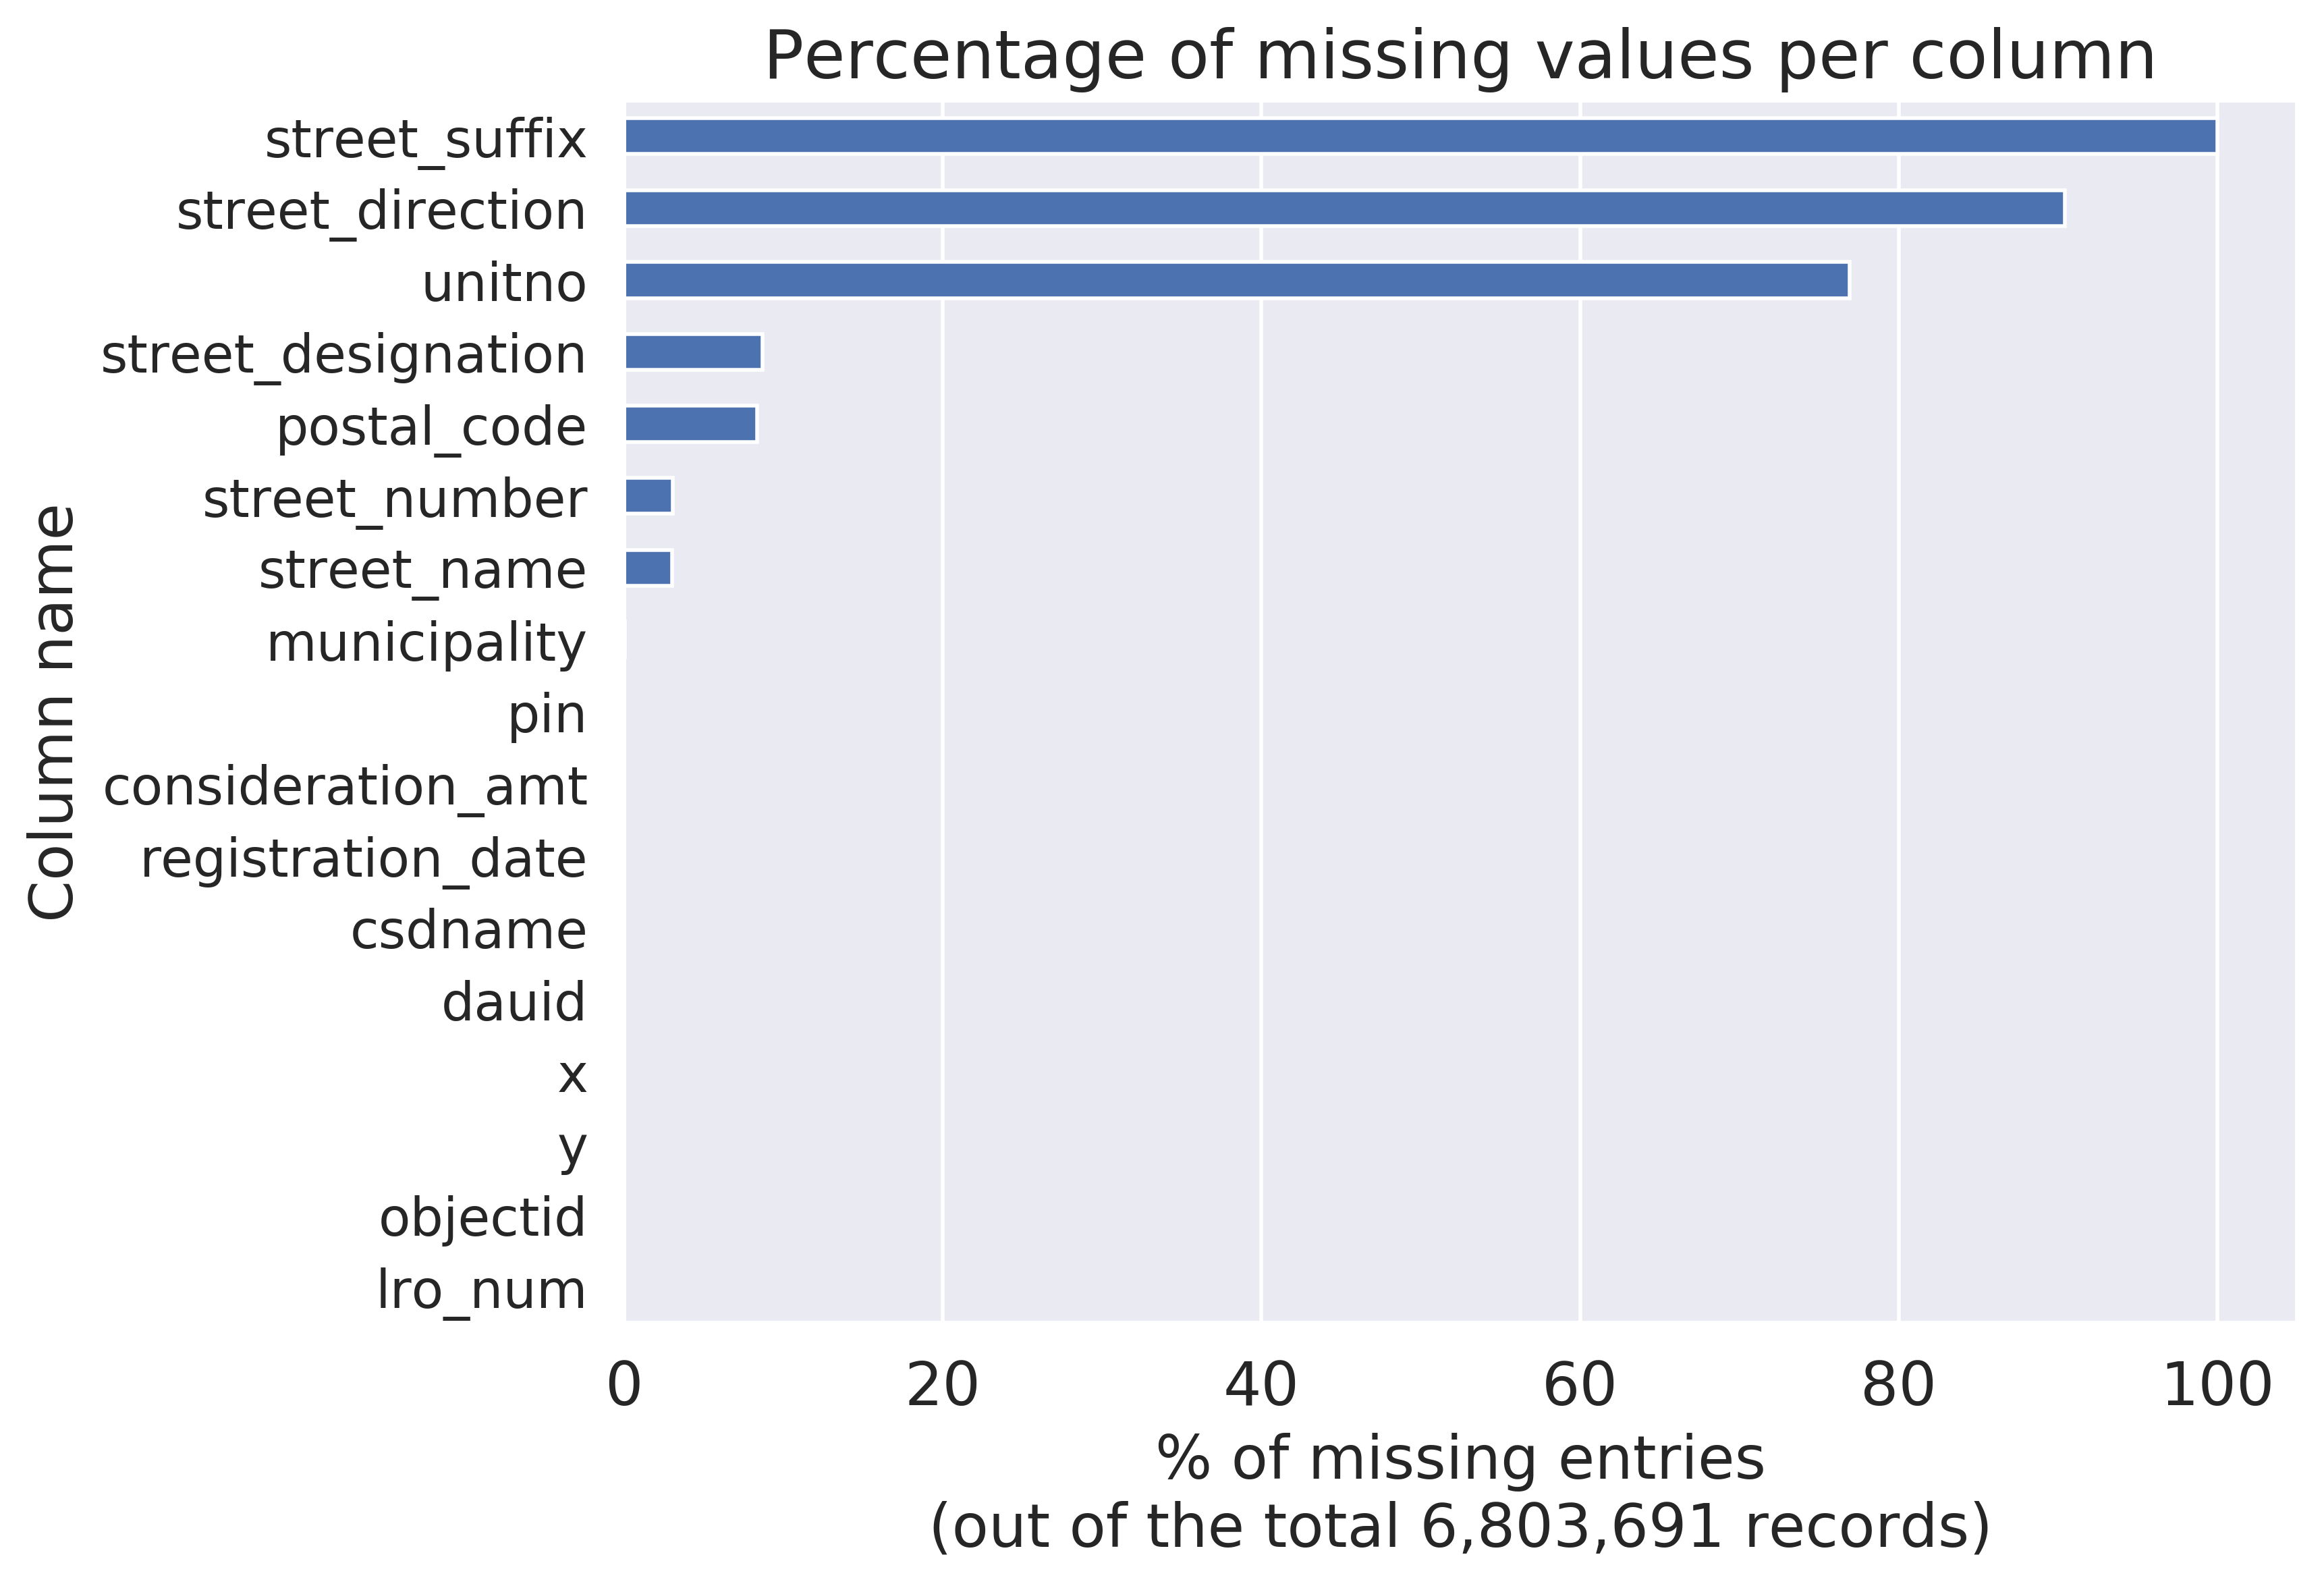
\includegraphics[width=1\linewidth,trim=1 1 1 1,clip]{img/teranet_na_perc.png}
        \caption{Missing values by column in the Teranet dataset (filtered to include only records with coordinates within GTHA boundary in Step 2.1).}
        \label{fig:teranet_na_counts}
    \end{figure}

    \newpage

    The following columns have most of the values present:

    \begin{itemize}
        \item \texttt{postal\_code} (8.37\% missing)
        \item \texttt{street\_name} (3.02\% missing)
        \item \texttt{street\_designation} (8.71\% missing)
        \item \texttt{municipality} (0.06\% missing)
        \item \texttt{street\_number} (3.08\% missing)
    \end{itemize}

    \vspace{5mm}

    The following columns have most of the values missing:

    \begin{itemize}
        \item \texttt{unitno} (76.9\% missing)
        \item \texttt{street\_direction} (90.4\% missing)
        \item \texttt{street\_suffix} (99.99994\% missing)
    \end{itemize}

    Since 99.99994\% of the values are missing in the column \texttt{street\_suffix}, it has been removed from the dataset.

    \subsubsection{Consistency of entries} \label{subsubsec:teranet_consistency}

    \begin{enumerate}
        \item \texttt{lro\_num} \textemdash consistent.
        No changes were made.
        \item \texttt{pin} \textemdash non-unique, but consistent.
        Unique \texttt{pin}s might or might not correspond to unique coordinate pairs (same coordinate pair can correspond to multiple unique \texttt{pin}s).
        No changes were made.
        \item \texttt{consideration\_amt} \textemdash consistent, but a large number of transactions have very low values of \texttt{consideration\_amt}, which appear to represent true recorded values (\textit{e.g.,} gift transactions).
        Also, outliers with very large \texttt{consideration\_amt} are present in the dataset, which also appear to represent true recorded values and correspond to high-value transactions of commercial property.
        \item \texttt{registration\_date} \textemdash consistent, one erratic entry was fixed in Step 2.2.
        \item \texttt{postal\_code} \textemdash consistent, converted to upper case as a preventive measure.
        Non-null values match the correct format for Canadian postal codes.
        \item \texttt{province} \textemdash consistent, removed from the Teranet dataset, as all the transactions are recorded in the Province of Ontario.
        \item \texttt{unitno} \textemdash some erratic values are present, fixed in Step 2.2.
        \item \texttt{street\_name} \textemdash some inconsistent values are present (different spellings of street names;
        with and without street designation;
        unit/suite number/postal code included;
        ''Highway'' or ''Hwy''; \textit{etc.}).
        Correcting all the values presents a time-intensive task, and thus was left for future targeted correction, capitalization were fixed in Step 2.2.
        \item \texttt{street\_designation} \textemdash some inconsistent values are present (\textit{e.g.,} ''St'', ''St W'', ''St.'', or ''Street''), most common problems were fixed in Step 2.2, capitalization were also fixed in Step 2.2.
        Street types were corrected in accordance to the list of recognized symbols and abbreviations provided by \textit{Canada Post}\cite{CanadaPost2019}.
        \item \texttt{street\_direction} \textemdash some inconsistent values are present (\textit{e.g.,} ''S'' and ''SOUTH''), fixed in Step 2.2.
        \item \texttt{municipality} \textemdash some inconsistent values are present (\textit{e.g.,} ''North York'' and ''North York/Toronto'', ''Hamilton'' and ''Hamilton City''), fixed in Step 2.2, capitalization were also fixed in Step 2.2.
        \item \texttt{street\_suffix} \textemdash all values are numeric, but consistent, very few values are non-null.
        As all the values are numeric, it is unclear how do they represent street suffix.
        \item \texttt{street\_number} \textemdash consistent, but some of the values are questionably large to represent a street number (\textit{e.g.,} 562916, 47626).
        \item \texttt{x} and \texttt{y} \textemdash consistent.
        Values appear to be in a reasonable range, but some coordinates clearly do not match the address/municipality, where the transaction is supposed to be recorded.
        However, majority of coordinate pairs appear to be reasonable.

        Records with coordinates that fall outside of the GTHA boundary, as specified by the geometry of the polygons of the GTHA Dissemination Areas, have been filtered out of the Teranet dataset via a spatial join in Step 2.1.
        Unique coordinate pairs might or might not correspond to unique \texttt{pin}s.
        There are more unique \texttt{pin}s than unique coordinate pairs (same coordinate pair can correspond to multiple unique \texttt{pin}s).
        No changes were made.
    \end{enumerate}

    \section{Step 2.3: Addition of new attributes} \label{sec:teranet_new_cols}

    Step 2.3 of the cleanup process for Teranet dataset focused on the addition of three more new attributes to each Teranet record (in addition to the three DA-level attributes that were added in Step 2.1).

    \vspace{5mm}

    Two new attributes were parsed from the values of \texttt{registration\_date} for grouping and visualization purposes:
    \begin{itemize}
        \item \texttt{year}
        \item \texttt{decade}
    \end{itemize}

    \vspace{5mm}

    A new attribute \texttt{transaction\_id} was added to provide unique identifier for Teranet records:
    \begin{itemize}
        \item No combination of native columns provides a convenient unique identification for Teranet records
        \item \texttt{pin}, \texttt{registration\_date}, \texttt{consideration\_amt}, \texttt{X} and \texttt{Y} coordinates, and other columns all have duplicate entries, and thus do not qualify as candidate keys
        \item A new column \texttt{transaction\_id} with a simple auto-incrementing range index (row number) will be added to provide a unique identifier for each Teranet record
        \item The new column \texttt{transaction\_id} captures the order of transactions in the Teranet dataset, previously filtered to include only transactions with coordinates that fall within the GTHA boundary (see Step 2.1), and ordered from earliest to latest \texttt{registration\_date}.
        \item The new column \texttt{transaction\_id} can be used as a Primary Key for Teranet table within the proposed Teranet database, and thus allows to take advantage of the indexing features available in PostgreSQL
    \end{itemize}

    \section{Step 2.4: Removal of duplicate records} \label{sec:teranet_drop_duplicates}

    \medskip

    \bibliography{teranet_cleanup_plan}
    \bibliographystyle{ieeetr}

\end{document}